\documentclass[12pt, preprint]{aastex}
\usepackage{bm}

\newcommand{\setof}[1]{\left\{{#1}\right\}}
\newcommand{\given}{\,|\,}
\newcommand{\dd}{\mathrm{d}}
\newcommand{\catalog}{\bm{Q}}
\newcommand{\pars}{\bm{\theta}}
\newcommand{\bs}[1]{\boldsymbol{#1}}

\newcommand{\Msun}{\ifmmode {M_{\odot}}\else${M_{\odot}}$\fi}

\begin{document}

\title{Modeling the X-Ray Populations of NGC 55}
\author{some combination of JJA, AZ, TF, and others}
\date{NOT READY}

\begin{abstract}
Really exciting abstract that will make everyone want to read this paper.
\end{abstract}

\section{Introduction}

{\it Chandra} has revolutionized our understanding of the x-ray emitting objects. It's unprecedented angular precision and collecting area allows it to identify dozens of resolved sources in nearby galaxies. Studies of individual objects have yielded a deeper insight into the physical processes forming the bulk of individually identified sources, low and high mass X-ray binaries (XRBs), as well as a rare, but important subset, the ultra-luminous X-ray sources (ULXs). High mass binaries, in particular, are formed from the accretion of an early-type star onto either a neutron star or black hole. Their relatively short lifetimes requires that these systems cannot travel far away from their birth site, and indeed observations show the majority of luminous X-ray sources are near star forming regions. 

NGC 55 is a relatively transparent, edge-on, nearby galaxy. Using the {\it Hubble Space Telescope}, and other optical telescopes, we have been able to identify a near-complete sample of star forming regions. For each region, multi-band photometry provides an estimate of the star formation history. 

In this work, we simulate the expected number, position, and characteristics of the X-ray binary population, given our sample of star forming regions, as well as the star formation history of the overall galaxy. We then apply a Bayesian method to generate a likelihood function comparing the resulting distribution with the observed X-ray sample.

\section{Method}

We begin with Bayes' Rule:
\begin{equation}
P( M \given D ) = \frac{P( D \given M ) P(M)}{P(D)},
\end{equation}
where $M$ is the model and $D$ is the data. In this case, $D$ includes the set of observed X-ray luminosities, companion masses (where available), and sky positions:
\begin{equation}
P ( D \given M ) = P( \bs{L_x}, \bs{M_2}, \bs{\alpha}, \bs{\delta} \given M),
\end{equation}
here we use bold quantities to identify sets of variables. The posterior probability over the entire set of observables is the product over the posterior probability over the observed quantities for each X-ray binary:
\begin{equation}
P( \bs{L_x}, \bs{M_2}, \bs{\alpha}, \bs{\delta} \given M) = \prod_i P( L_x, M_2, \alpha, \delta \given M).
\end{equation}
We now marginalize over the birth time ($t_b$), the birth kick velocity ($v_k$), and from which star forming region each system was formed ($C$):
\begin{equation}
P( L_x, M_2, \alpha, \delta \given M) = \sum_{{\rm all}\ C} \int \int P( L_x, M_2, \alpha, \delta, t_b, C, v_k \given M)\ \dd v_k\ \dd t_b\ \dd C.
\end{equation}
There are an integer number of star forming regions, so we expressed the integral over $C$ as a sum over the known set of star forming regions. This assumes a complete census of the star forming regions in NGC 55. ({\bf Is this reasonable? If not, we should add a complication to the model to account for our non-perfect knowledge.}). Based on independence, we can separate out several terms:
\begin{equation}
\sum_{{\rm all}\ C} \int \int P(\alpha, \delta \given v_k, C, t_b) P(L_x, M_2, v_k \given t_b, M)\ \dd v_k\ P(t_b \given C)\ \dd t_b.
\end{equation}
We discuss each of these terms in turn. 

The first term provides the probability that, given a birth time, kick velocity, and particular star forming region, what is the probability that the X-ray binary would be observed at its current position. For the vast majority of parameter space, this probability is zero. For example, given a short birth time, and a small kick velocity, none but the nearest star forming regions could have formed that particular system. We can only observe the projected distance between the X-ray binary and its candidate host star forming region. The actual distance is $v_k t_b$. We care only about the distance the cluster is from each particular star forming region, so the probability is equal to the probability of the X-ray binary being ejected from that particular star forming region along the angle implied by the distance traveled $v_k t_b$ and the projected separation $s$. This probability is equal to the probability of randomly drawing a polar angle (multiplied by two since the X-ray binary could be either in front of or behind the star forming region:
\begin{equation}
P(\alpha, \delta \given v_k, C, t_b) = \frac{s}{v_k t_b}.
\end{equation}

Given a birth time and a particular binary population synthesis model, the second term provides the probability that a binary with a particular $L_x$, $M_2$, and $v_k$ will be formed. We discuss this term in detail below.

The final term gives the probability of a birth time for a particular cluster. The birth time probability is directly related to the star formation rate at that time:
\begin{equation}
P(t_b \given C) \propto \dot{M}(t_b).
\end{equation} 
Determining this term therefore requires a knowledge of the star formation history of each star forming cluster. Multi wavelength observations have allowed approximate knowledge of the star formation histories for most of the star forming regions in NGC 55, at least within the recent past.

 
 
\section{Calculating $P(L_x, M_2, v_k \given t_b, M)$}

We choose to adapt and improve upon the Jacobian formalism discussed by Ghosh et al.\ over several papers. The underlying premise relies upon our ability to map the initial state of a binary through its various stages, until it forms an X-ray luminous object. If this can be done analytically or semi-analytically, such that the derivatives of these mappings can be calculated, then the Jacobian matrices of these mappings can be used to determine the probability of finding any particular binary at any stage of its evolution from its corresponding initial conditions alone.


As opposed to this semi-analytic formalism, population synthesis traditionally opts for Monte Carlo methods. There is a simple reason for this: Monte Carlo methods require only an initial distribution of binaries and an understanding of how any particular system evolves from its initial state. This lends itself well to evolving systems through complex physical processes that require numerical integration. Jacobian transformations, on the other hand require knowledge of the initial parameters of systems that form the end-state binaries in question. Or put another way, Monte Carlo modeling requires only the forward mapping, while Jacobian transformations require the backward mapping (as well as its first derivatives). Therefore, binary population studies have traditionally focused on Monte Carlo modeling. The downside is that, since the reverse mapping does not exist, there is no information {\it a priori} about which initial binaries will evolve into those in question, Monte Carlo population synthesis often requires generating some 10$^6$ random initial binaries to accurately cover the large dimensional initial phase space.
%The reasons for this are many: including complex physics is much easier using Monte Carlo methods, the Jacobian transformation method requires the transformations to be analytic or semi-analytic whereas certain physical processes require numerical integration to accurately calculate, and Monte Carlo methods can easily handle complicated evolutionary channels. 
The computation time required can be considerable. Parameter studies are therefore often limited to a few key physical aspects, typically testing tens to hundreds of separate models. Figure \ref{fig:Mapping} shows an abstract demonstration of the transformation from the initial binary through the first (stable) mass transfer phase ($G_{\rm MT}$) the through the primary's core collapse ($H_{\rm SN}$), and finally into the observed X-ray luminous phase once the secondary star feeds the NS from a stellar wind ($I_{\rm XRB}$).

\begin{figure}[h!]
\begin{center}
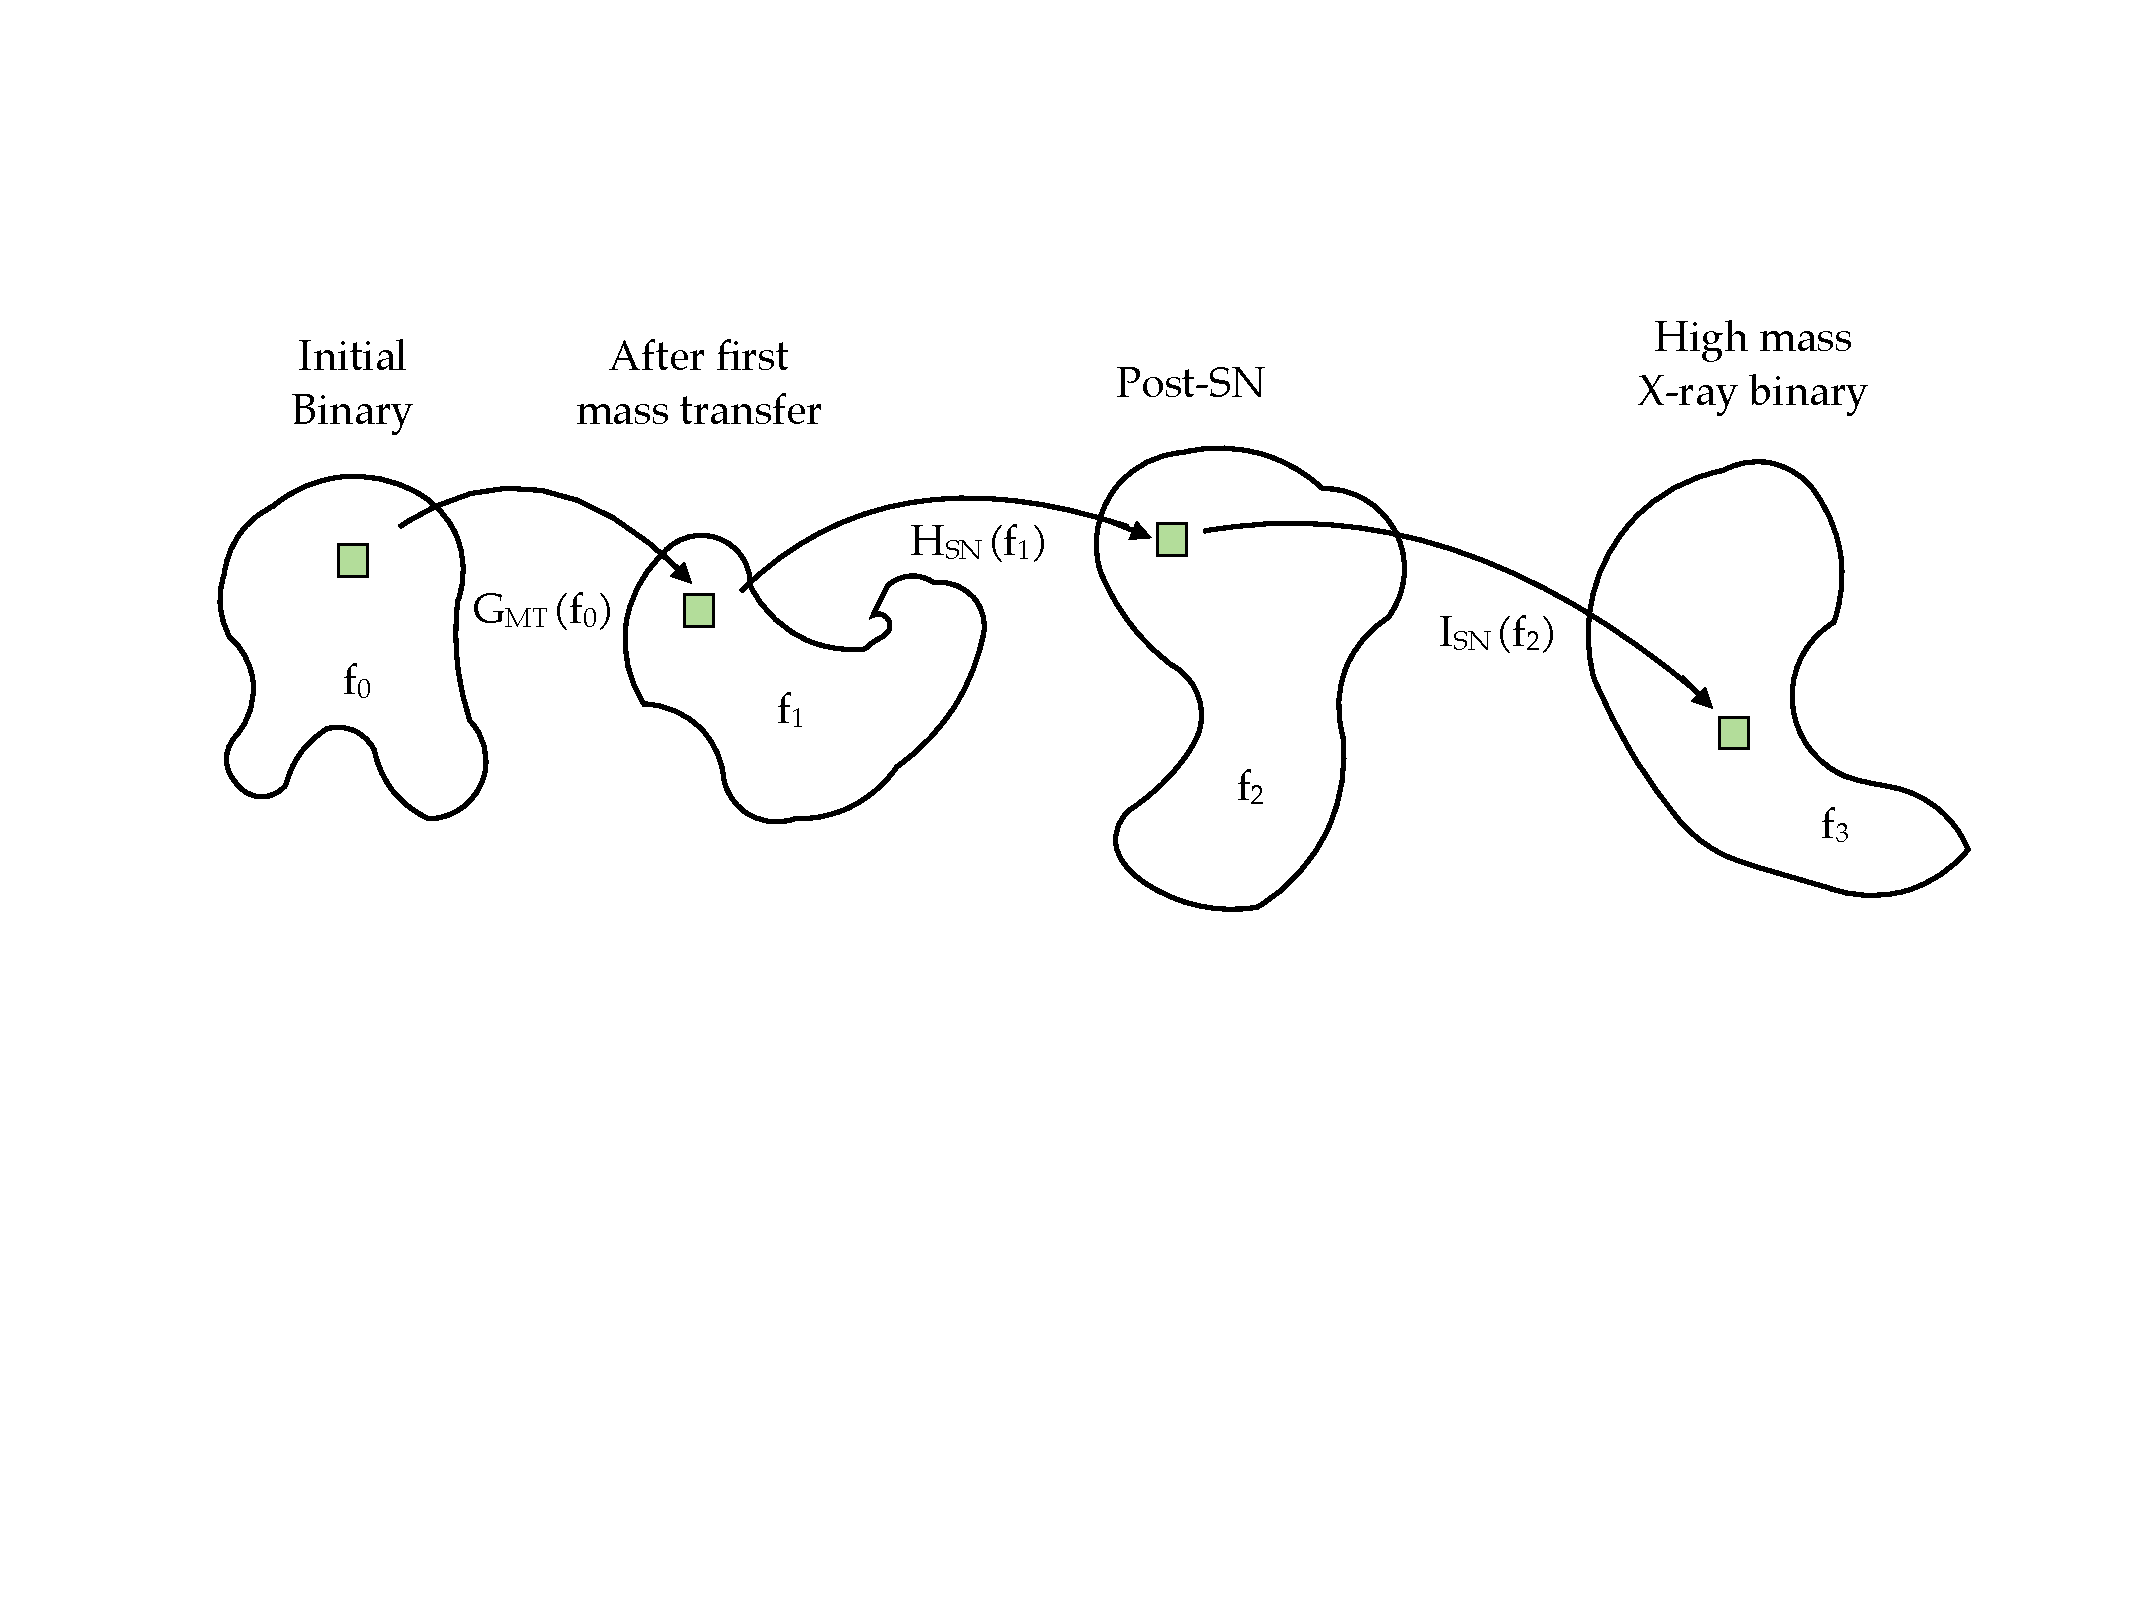
\includegraphics[width=0.95\columnwidth]{Mapping.pdf}
\caption{A mathematical representation of the evolution of a binary from its initial state three separate stages of evolution: the first (stable) mass transfer phase ($G_{\rm MT}$), the primary undergoing core collapse and receiving a natal kick ($H_{\rm SN}$), and the X-ray luminous phase once the second star evolves off the main sequence ($I_{\rm XRB}$). The volume of the six dimensional box around the binary scales with the determinant of the Jacobian matrix for each mapping.}
\label{fig:Mapping}
\end{center}
\end{figure}

Mathematically, these mappings can be expressed in a straightforward way:
\begin{eqnarray}
f_1 &=& G_{\rm MT} (f_{\rm primo}) \\
f_2 &=& H_{\rm SN} (f_1) \\
f_3 &=& I_{\rm XRB} (f_2). \\
\end{eqnarray}
These can be combined:
\begin{equation}
f_3 = I_{\rm XRB}\{ H_{\rm SN}[ G_{\rm MT} ( f_{\rm primo}) ] \}.
\end{equation}

If, however, a reverse mapping exists or it can be determined numerically, then the problem is greatly simplified. This mapping allows one to determine the initial binary state of the observed system:
\begin{equation}
f_{\rm primo} = G_{\rm MT}^{-1} \{ H_{\rm SN}^{-1} [ I_{\rm XRB} (f_3) ] \}.
\end{equation}
Determining the probability of the observed binary is now straightforward:
\begin{eqnarray}
P(f_3) &=& P(f_2) | J_{\rm XRB} | \\
  &=& P(f_1) | J_{\rm SN} | | J_{\rm XRB} | \\
  &=& P(f_{\rm primo}) | J_{\rm MT} | | J_{\rm SN} | | J_{\rm XRB} |.
\end{eqnarray}
Our model provides the probability of the initial state of the binary, $P(f_{\rm primo})$. Now we need to determine the probabilities of the Jacobian determinants for each of the three physical processes. We discuss each of these in turn below.


The Jacobian transformations require one-to-one mappings, yet even the most ideal observations of high mass X-ray binaries are unlikely to identify enough parameters to uniquely determine any particular system's prior evolution. To determine the probability of any model producing a binary with observed parameters ($\vec{x}$) we marginalize over latent unobserved parameters ($\vec{y}$):
\begin{equation}
P[f_{\rm obs}(\vec{x})] = \int P[f_3(\vec{x}, \vec{y})] \dd \vec{y}
\end{equation}


%Since we are only interested in a small subset of binaries, those that are strong X-ray sources, we can employ the Jacobian transformation method here. The nature of the method is significantly computational cheaper since the region of parameter space explored is, by design, limited to only those binaries we are interested in.



\subsection{The First Mass Transfer Phase}

We start with the initial conditions of the binary, which includes six parameters, the primary mass ($M_1$), the secondary mass ($M_2$), the orbital separation ($A$), the SN kick velocity ($v_k$), the kick polar angle ($\theta$), and the kick azimuthal angle ($\phi$). Although the three SN kick parameters are not explicitly relevant for the initial state of the binary, they become relevant when calculating the post-SN orbit:
\begin{equation}
f_{\rm primo} = P(M_1, M_2, A, v_k, \theta, \phi).
\end{equation}


Once the first star evolves past its main sequence onto the giant branch, it begins overfilling its Roche lobe. We select only those systems that will undergo stable mass accretion, which can be determined by comparing the thermal time of the secondary with the mass accretion time. This comparison determines whether the transferring matter can lose its entropy fast enough to become incorporated with the companion star, or whether it forms a common envelope. The mapping from the initial binary conditions to the post-mass transfer binary is straightforward. The post mass transfer primary becomes the primary core mass ($M_{1,c}$), while the secondary incorporates the primary's lost envelope. From Ghosh et al.: 
\begin{eqnarray} 
M_1' &=& M_{1,c} \\
M_2' &=& M_1 + M_2 - M_{1,c},
\end{eqnarray}
and
\begin{equation}
A' = A \left[ \frac{M_1 M_2}{M_1' M_2'} \right]^2.
\end{equation}
$M_{1,c}$ can be estimated by:
\begin{equation}
M_{1,c} = M_0 M_1^{1/\xi},
\end{equation}
where $M_0 = 0.073 \Msun$ and $\xi = 0.704 \Msun$. Determining the Jacobian matrix of this transformation (which we provide in the appendix) allows us transform the initial binary distribution into the post mass transfer distribution:
\begin{equation}
P(M_1, M_2, A, v_k, \theta, \phi) = P(M_1', M_2', A', v_k, \theta, \phi) J_{MT}.
\end{equation}
We assume that the binary does not change between the end of the mass transfer phase until the primary undergoes a SN. 


We next calculate the post-SN orbital separation ($A''$), systemic velocity ($v_{\rm sys}$), and eccentricity ($e$) based on the equations in Kalogera (1996):
\begin{eqnarray}
A'' &=& GM_1M_2 \left[ -\left( \frac{M_1''M_2''}{M_1'' + M_2''} \right) v_1^2 + \frac{2GM_1''M_2''}{A'} \right] ^{-1} \label{eq:SN_A} \\
v_{\rm sys} &=& \left( \frac{M_1''}{M_1'' + M_2''} \right) \sqrt{ |v_1^2| } \label{eq:SN_v_sys} \\
1-e^2 &=& \frac{A'^2}{A'' \mu} \left[ v_k^2 \cos^2\theta + v_k^2 \sin^2 \theta \sin^2 \phi + v_k \left( \frac{\mu}{h} \right) \cos \theta + \left( \frac{\mu}{h} \right)^2  \right], \label{eq:SN_e}
\end{eqnarray}
where $\mu = G(M_1' + M_2')$, $\mu/h = \sqrt{G(M_1'+M_2') / A'}$, and $v_1$ is the orbital velocity of the primary just prior to SN:
\begin{equation}
v_1^2 = v_k \left( \frac{\mu}{h} \right) \cos \theta + v_k^2 + \left( \frac{\mu}{h} \right)^2. 
\end{equation}
Derivatives of equations \ref{eq:SN_A}, \ref{eq:SN_v_sys}, and \ref{eq:SN_e} determine the Jacobian $J_{\rm SN}$. We provide the analytic form for $J_{\rm SN}$ in the Appendix. The probability of the post-SN parameters from the pre-SN parameters and the three kick parameters is:
\begin{equation}
P(M_1'', M_2'', A'', v_k, v_{\rm sys}, e) = P(M_1', M_2', A', v_k, \theta, \phi) J_{\rm SN}.
\end{equation}


Once the secondary evolves onto the core helium burning branch, its luminosity increases, and the star emits a wind accreted by the primary NS. Determining the X-ray luminosity ($L_x$) from the accretion rate ($\dot{M}$) is straightforward: 
\begin{equation}
L = \frac{G M_{\rm NS} \dot{M}}{R_{\rm NS}}.
\end{equation}
Now, we must determine $\dot{M}$ as a function of orbital parameters.




\section{Experiments}

... Make a test model to check our code and see if it actually works.

\section{Results}

... Apply our model to the data from NGC 55. 

\section{Discussion}

... First stab at a difficult problem. This is the basics, but generalization to X-ray populations in all galaxies should be possible.

... What does this imply about our understanding of NGC 55? What about binary population synthesis? Kick velocities? High mass binary evolution?

\acknowledgements
It is a pleasure to thank...
Funding...
Code...

\end{document}
